\documentclass{article}
\usepackage{amsmath}
\usepackage{graphicx}
\usepackage{fullpage}

\title{10-703 Deep Reinforcement Learning and Control \\ Assignment 2 \\}
\date{}

\setlength\parindent{0pt}

\begin{document}

\maketitle

\section{Proof}
Update (1) updates $Q(s,a)$ with $\alpha \Delta Q(s,a)$, where
\begin{align}
  \label{eq:1}
  \Delta Q(s,a) = r + \gamma \max_{a' \in A} Q(s', a') - Q(s,a)
\end{align}

Update (2) updates $w$ with $\alpha \Delta w$, where
\begin{align}
  \label{eq:2}
  \Delta w &= (r + \gamma \max_{a' \in A} Q(s', a') - Q(s,a)) \nabla_{w} Q_{w}(s,a) \\
           &= \Delta Q(s,a) \nabla_{w} Q_{w}(s,a) 
\end{align}

Proving two updates are the same is equivalent to proving
\begin{align}
  \label{eq:3}
  \Delta Q(s,a) = Q_{w+\Delta w}(s,a) - Q_{w}(s,a) 
\end{align}

The RHS is 
\begin{align}
  \label{eq:4}
  Q_{w+\Delta w}(s,a) - Q_{w}(s,a) &= (w + \Delta w)^{T} \phi(s,a) - w^{T} \phi(s,a) \\
                                   &= \Delta w^{T} \phi(s,a) \\
\end{align}

According to \eqref{eq:2},
\begin{align}
  \label{eq:5}
  Q_{w+\Delta w}(s,a) - Q_{w}(s,a) = \Delta Q(s,a) (\nabla_{w} Q_{w}(s,a))^{T} \phi(s,a)\\
\end{align}

While,
\begin{align}
  \label{eq:6}
  \nabla_{w} Q_{w}(s,a) = \nabla_{w} w^{T}\phi(s,a) = \phi(s,a)^{T}
\end{align}

Thus,
\begin{align}
  \label{eq:7}
  Q_{w+\Delta w}(s,a) - Q_{w}(s,a) = \Delta Q(s,a) \phi(s,a)^{T} \phi(s,a)
\end{align}

Given $(s,a)$, $\phi(s,a)$ is an one-hot vector, so $\phi(s,a)^{T} \phi(s,a) = 1$.

Thus, $Q_{w+\Delta w}(s,a) - Q_{w}(s,a) = \Delta Q(s,a)$. 

\section{Experimental Setup}
We ran all the experiments on SpaceInvaders-v0. The experimental setup is detailed below:

\subsection{Hyper Parameters}
We closely follow the parameters from the reference papers for all of our experiments, which are listed below: \\

Discount factor $\gamma$: 0.99\\
Learning rate $\alpha$: 0.0001\\
Epsilon decay policy: start with $\epsilon$=1 and drop it to 0.1 over 1000000 iterations\\
Iterations: 5000000\\
Number of frames to feed: 4\\
Input image size: 84 x 84 x 1\\
Replay buffer size: 1000000\\
Target Q-network reset interval: 10000\\
Batch size: 32\\
Train interval: 4

\subsection{Optimization}
We use {\em Huber loss} as the training loss and {\em Adam} as the optimizer. 

\subsection{Evaluation} 
To evaluate the performance over training, we periodically (every 10000 updates) run the learned policy for 20 episodes and average the total reward. During evaluation we use an epsilon-greedy policy with epsilon equal to 0.05. 

\subsection{Architectures}

We implemented six Q-networks in this assignment, including:
\begin{itemize}
\item Linear Q-Network without experience replay or target fixing (Linear*)
\item Linear Q-Network (Linear*) 
\item Double Linear Q-Network (Double-Linear-Q)
\item Deep Q-Network
\item Double Deep Q-Network
\item Dueling Deep Q-Network
\end{itemize}

\subsubsection{Linear Q-Networks}
For all {\em linear} Q-networks, we implement with a perceptron, which is a fully connected layer mapping 84x84x4 input to 6 actions. When implementing double linear Q-networks, we create two models with the same architecture described above, and randomly choose one network to set target Q and update the other network to minimize the distance between its predicted Q and the target Q.

\subsubsection{Deep Q-Networks} 
{\bf DQN:} The input to the deep Q-network consists of an 84x84x4 image. The first hidden layer convolves 16 8x8 filters with stride 4 and applies a rectifier nonlinearity. The second layer convolves 32 4x4 filters with stride 2 also followed by rectifier nonlinearity. The final layer is fully connected and consists of 256 rectifier unit. The output layer is a fully connected linear layer with a single output for each action. In case of SpaceInvaders the number of actions is 6.

{\bf Double-DQN:} The network architecture we used for double-DQN is the same as we used for DQN. The key algorithmic difference is that it decouples the action selection and evaluation steps to prevent overestimations.

{\bf Dueling-DQN:} The first three hidden layers for the dueling-DQN are the same as the model we used for DQN. After that the dueling network splits the model into two streams to separately estimate the state-value and the advantages for each action and the two sets of values are finally combined to get the Q-values at the output.

% \section{Implement the deep Q-network}
% \subsection{Network model}


% \section{Implement the double deep Q-network}
% \subsection{Network model}


% \section{Implement the dueling deep Q-network}
% \subsection{Network model}


\section{Experimental Results}

\subsection{Performance over training}
We show the performance over training for all {\em linear} Q-networks in Figure~\ref{fig:linear-simple},~\ref{fig:linear}, and~\ref{fig:double-linear}. We show the performance over training for all {\em deep} Q-networks in Figure~\ref{fig:dqn},~\ref{fig:double}, and~\ref{fig:duel}. 
\begin{figure}[h]
\centering
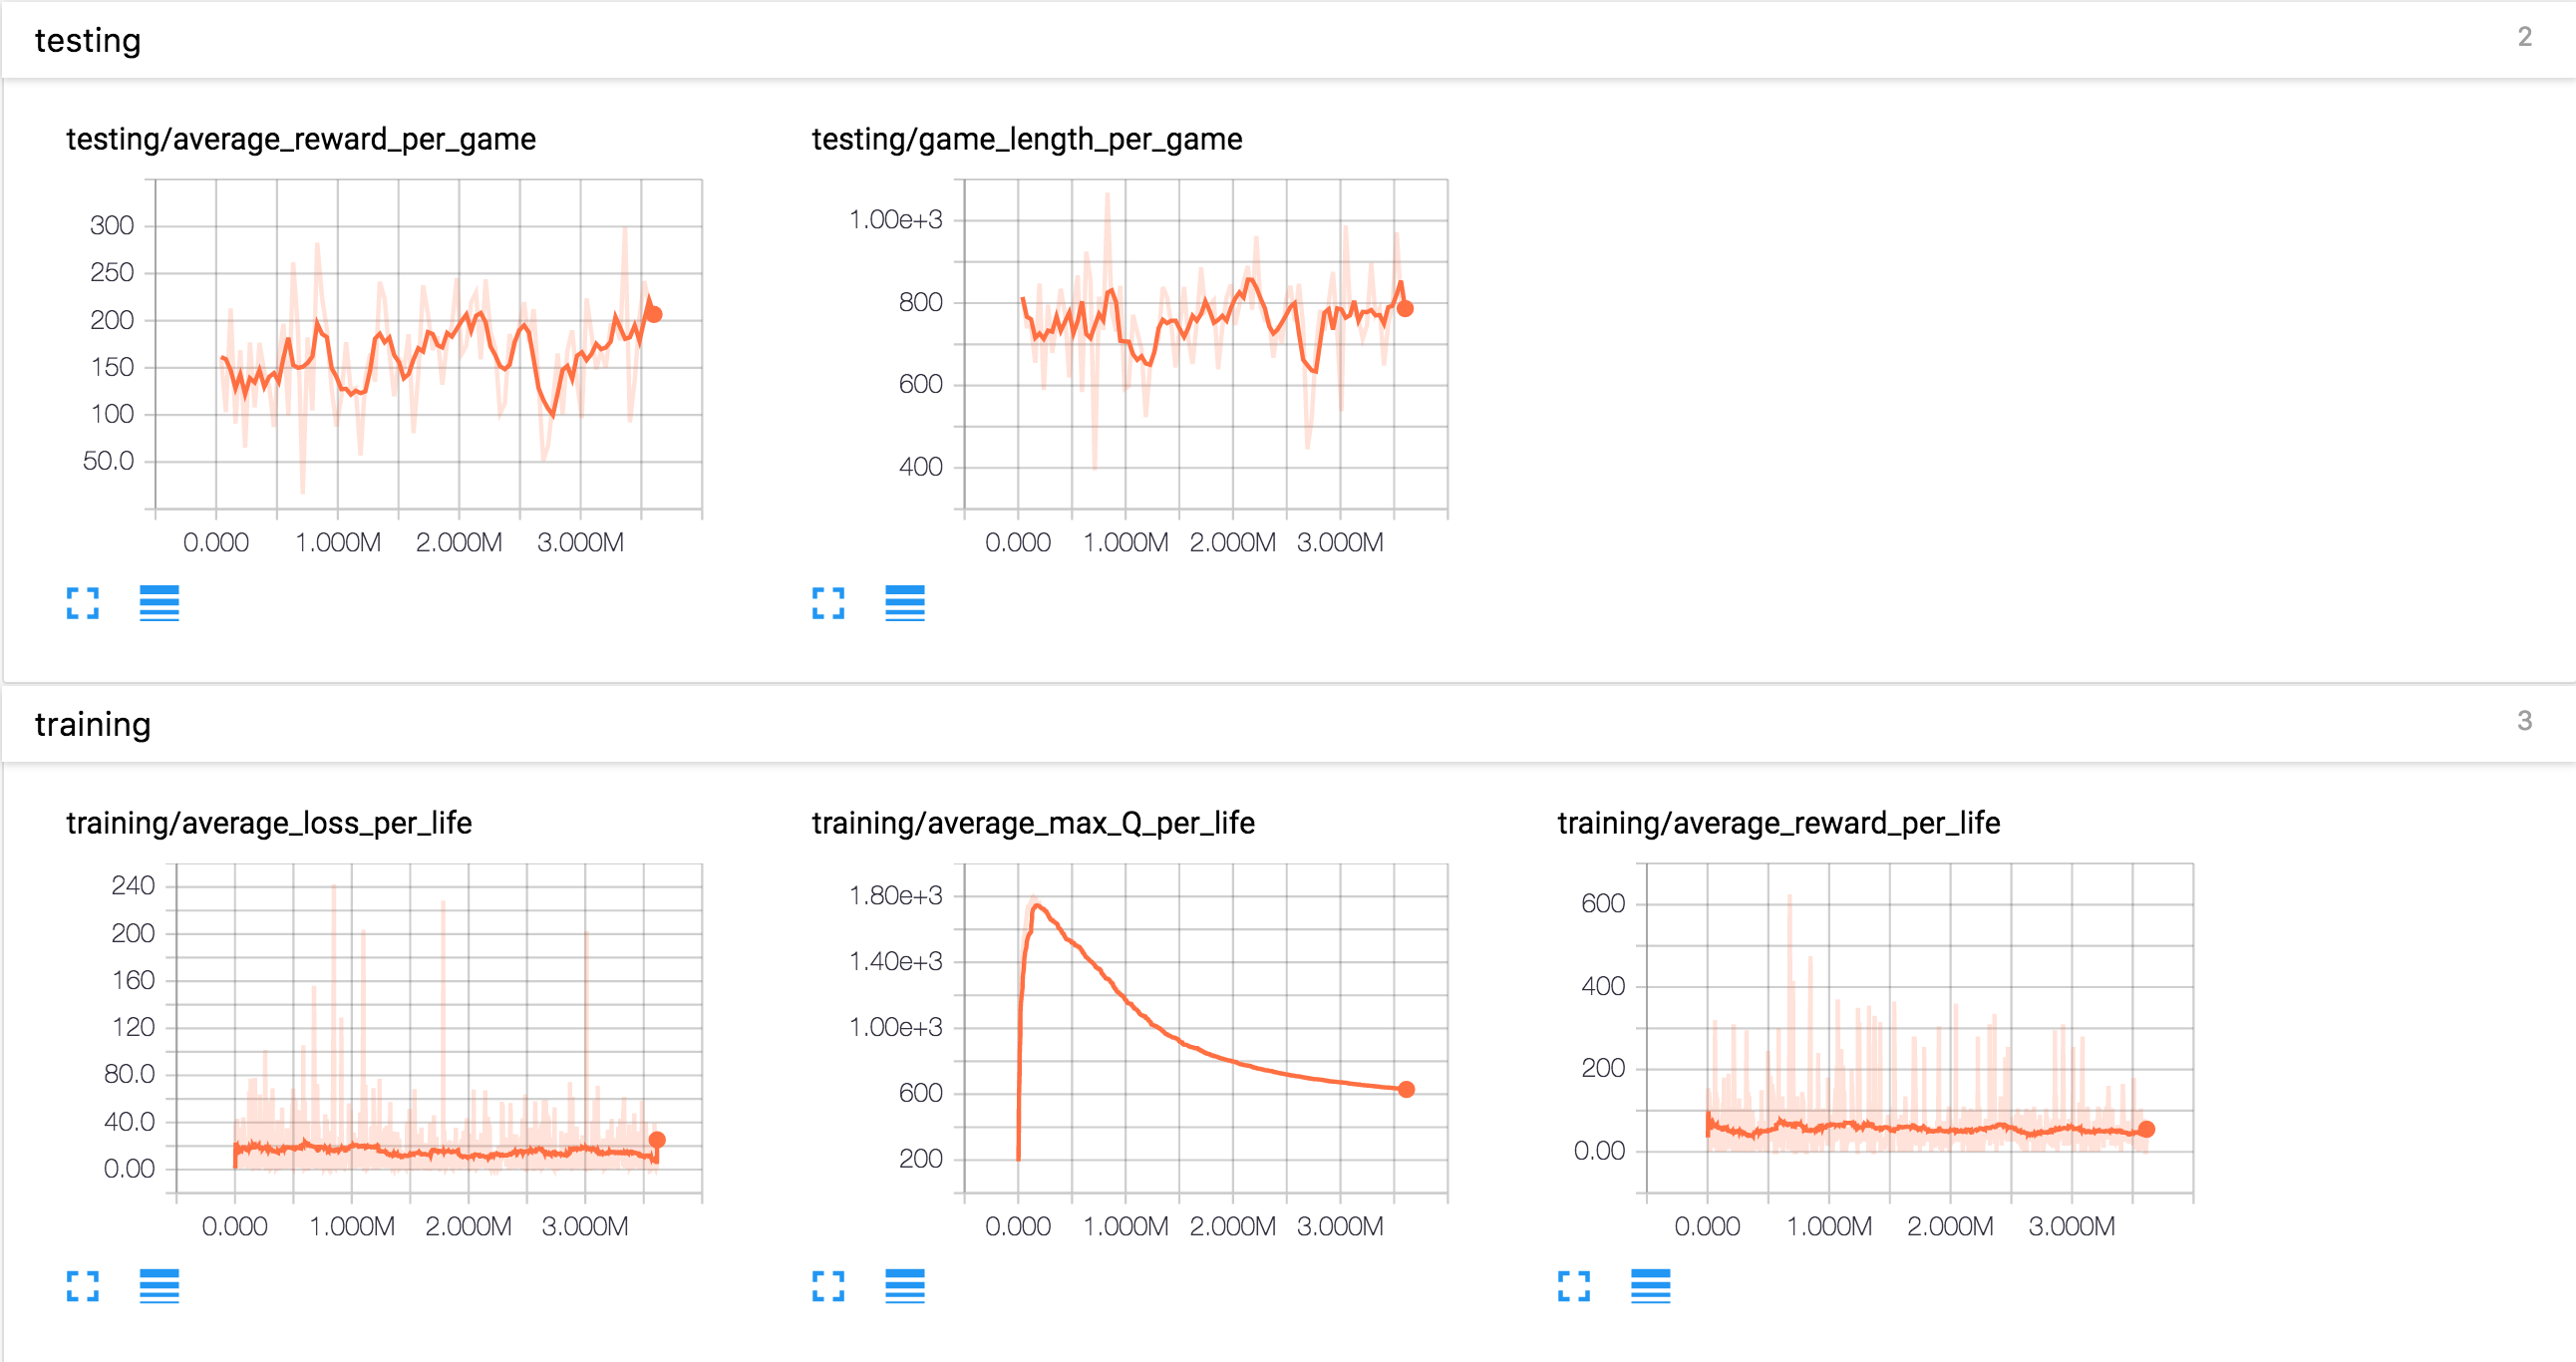
\includegraphics[width=\linewidth]{plots/linear_simple.png}
\caption{{\em Linear Q-Network with {\bf no} experience replay or target fixing:} The progression of max Q value is unexpected - it goes up quickly in the early training stage and then gradually dive down. The behavior is likely due to no access to experience replay or target fixing, since the Q-network updates based on a single sample of experience every iteration. There is no noticeable improvement over time in the average reward plot. }
\label{fig:linear-simple}
\end{figure}

\begin{figure}[h]
\centering
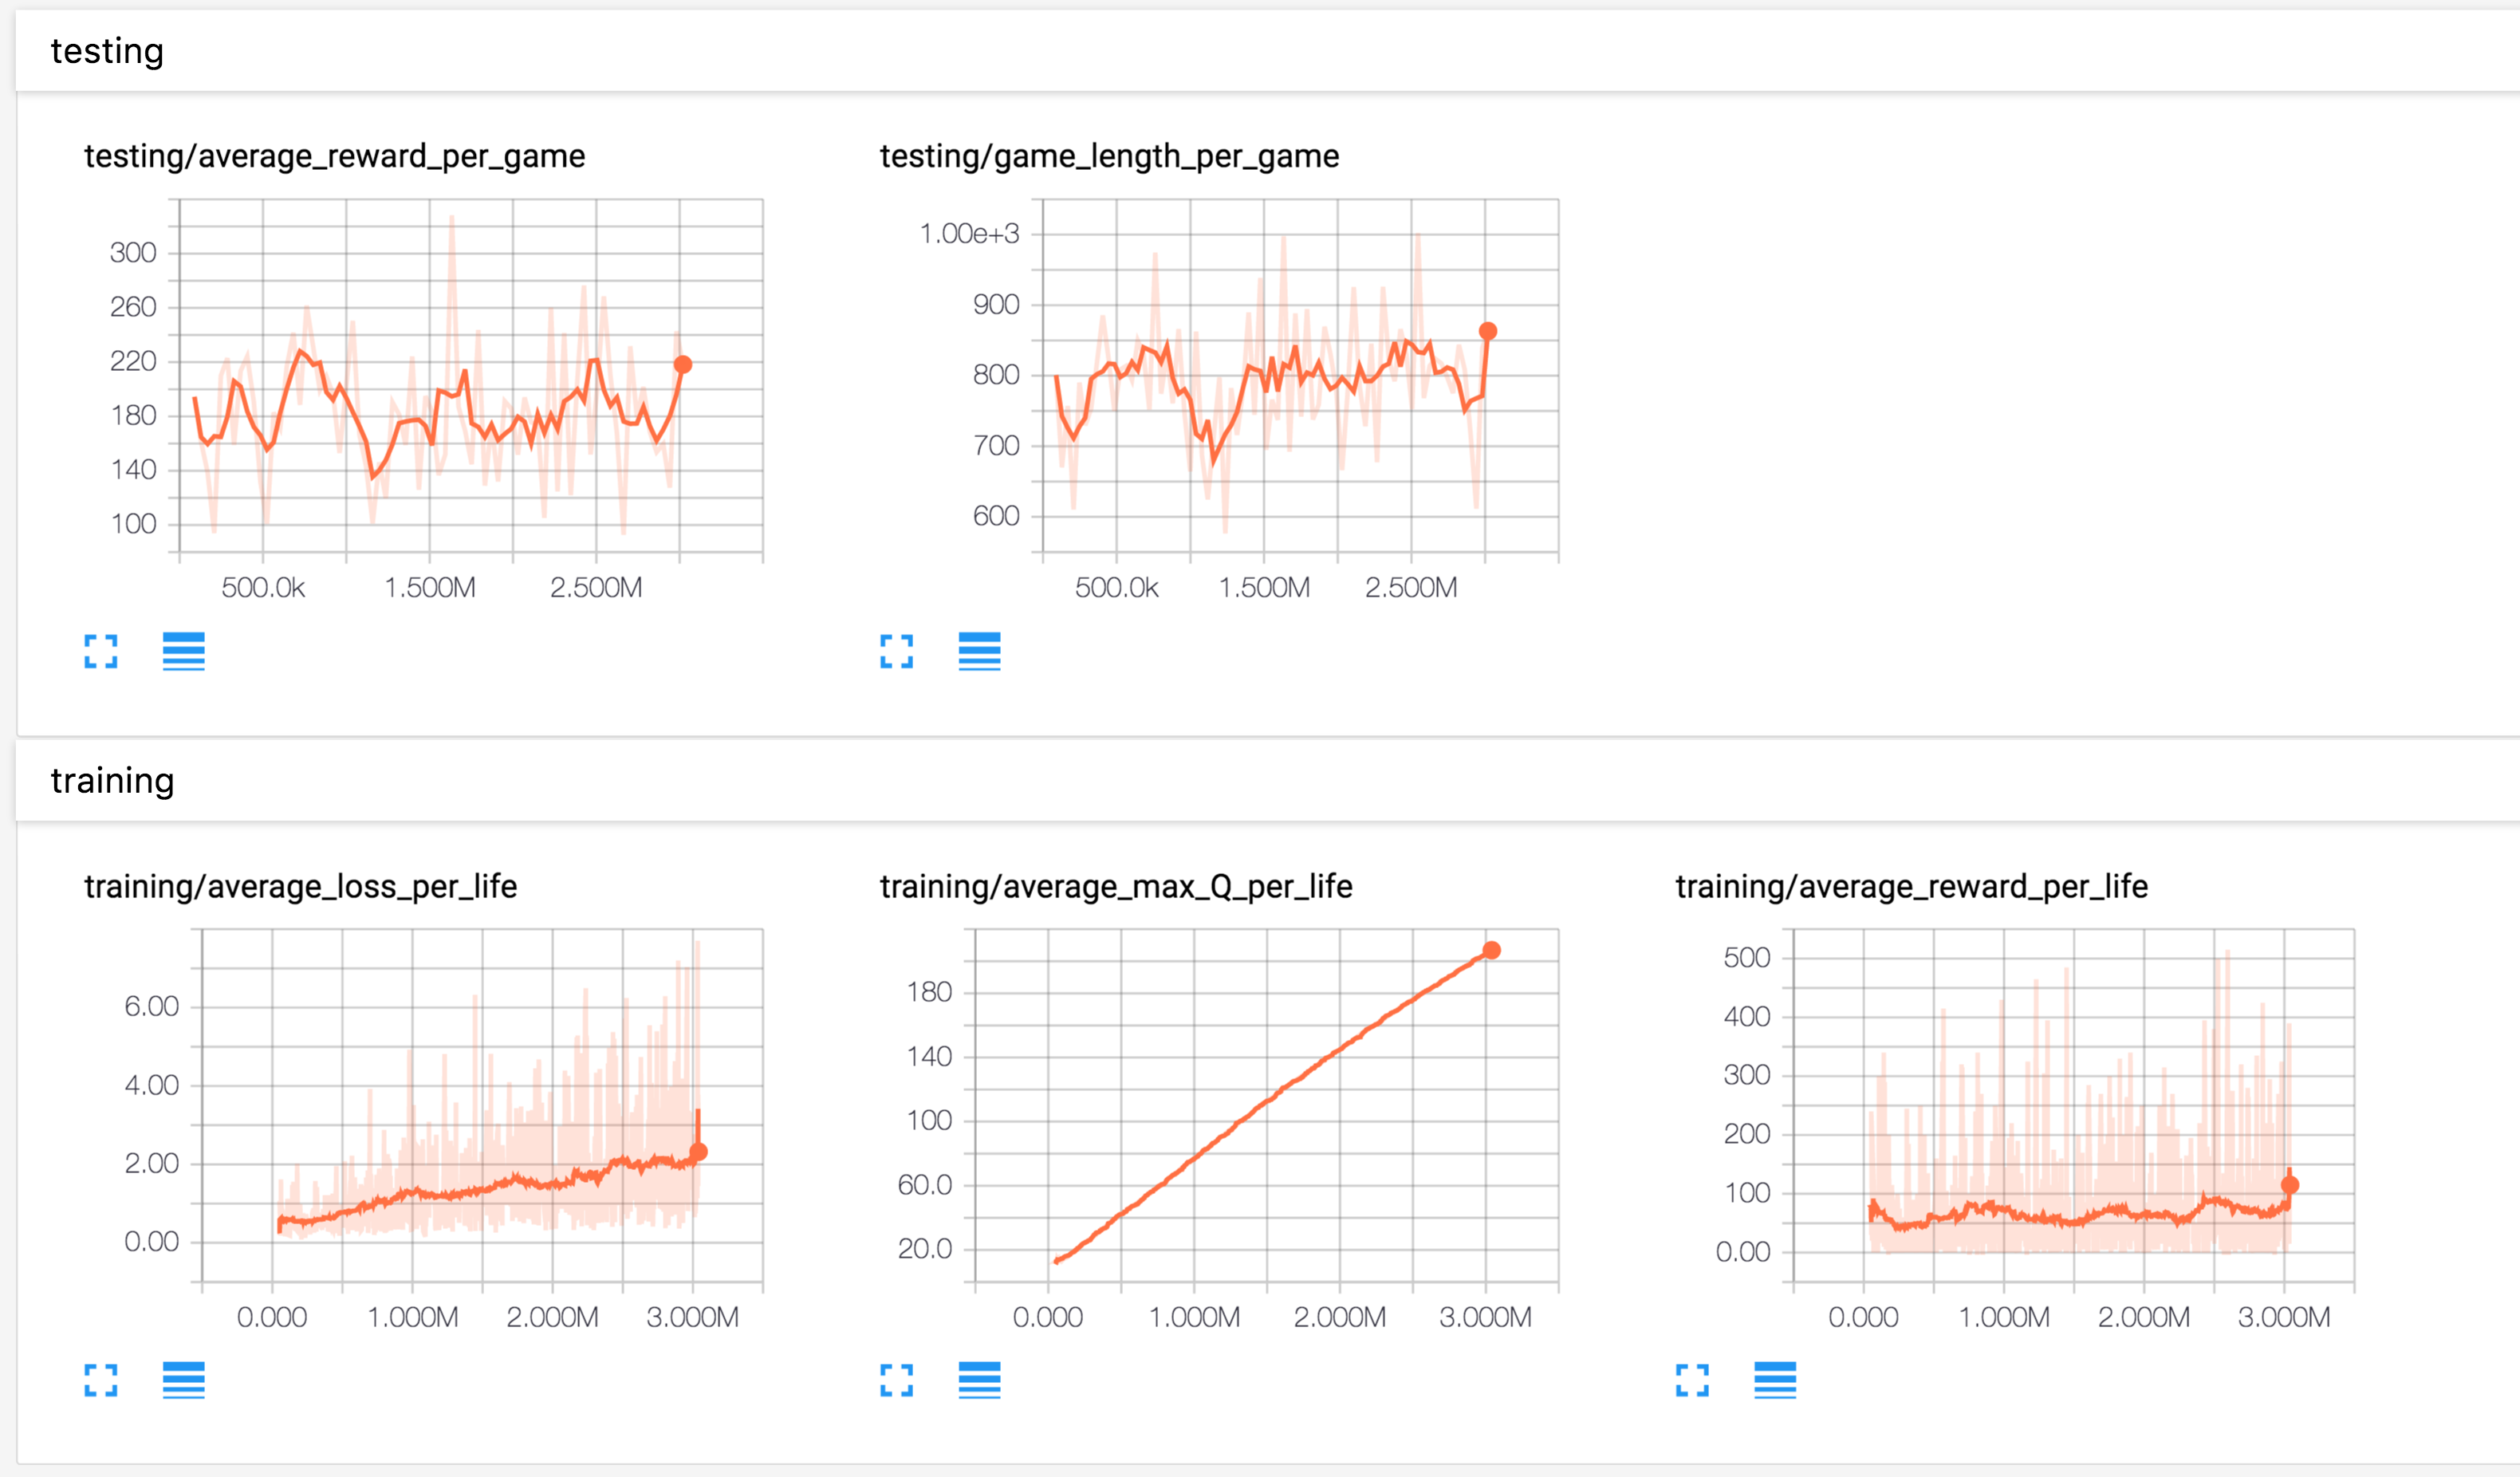
\includegraphics[width=\linewidth]{plots/linear.png}
\caption{{\em Linear Q-Network with experience replay and target fixing:} The progress of max Q value looks more reasonable than the one in Figure~\ref{fig:linear-simple}, since it observes better chances of achieving higher rewards as it gathers more experiences. Also, we are now able to observe stable improvement in average reward over the training process. } 
\label{fig:linear}
\end{figure}

\begin{figure}[h]
\centering
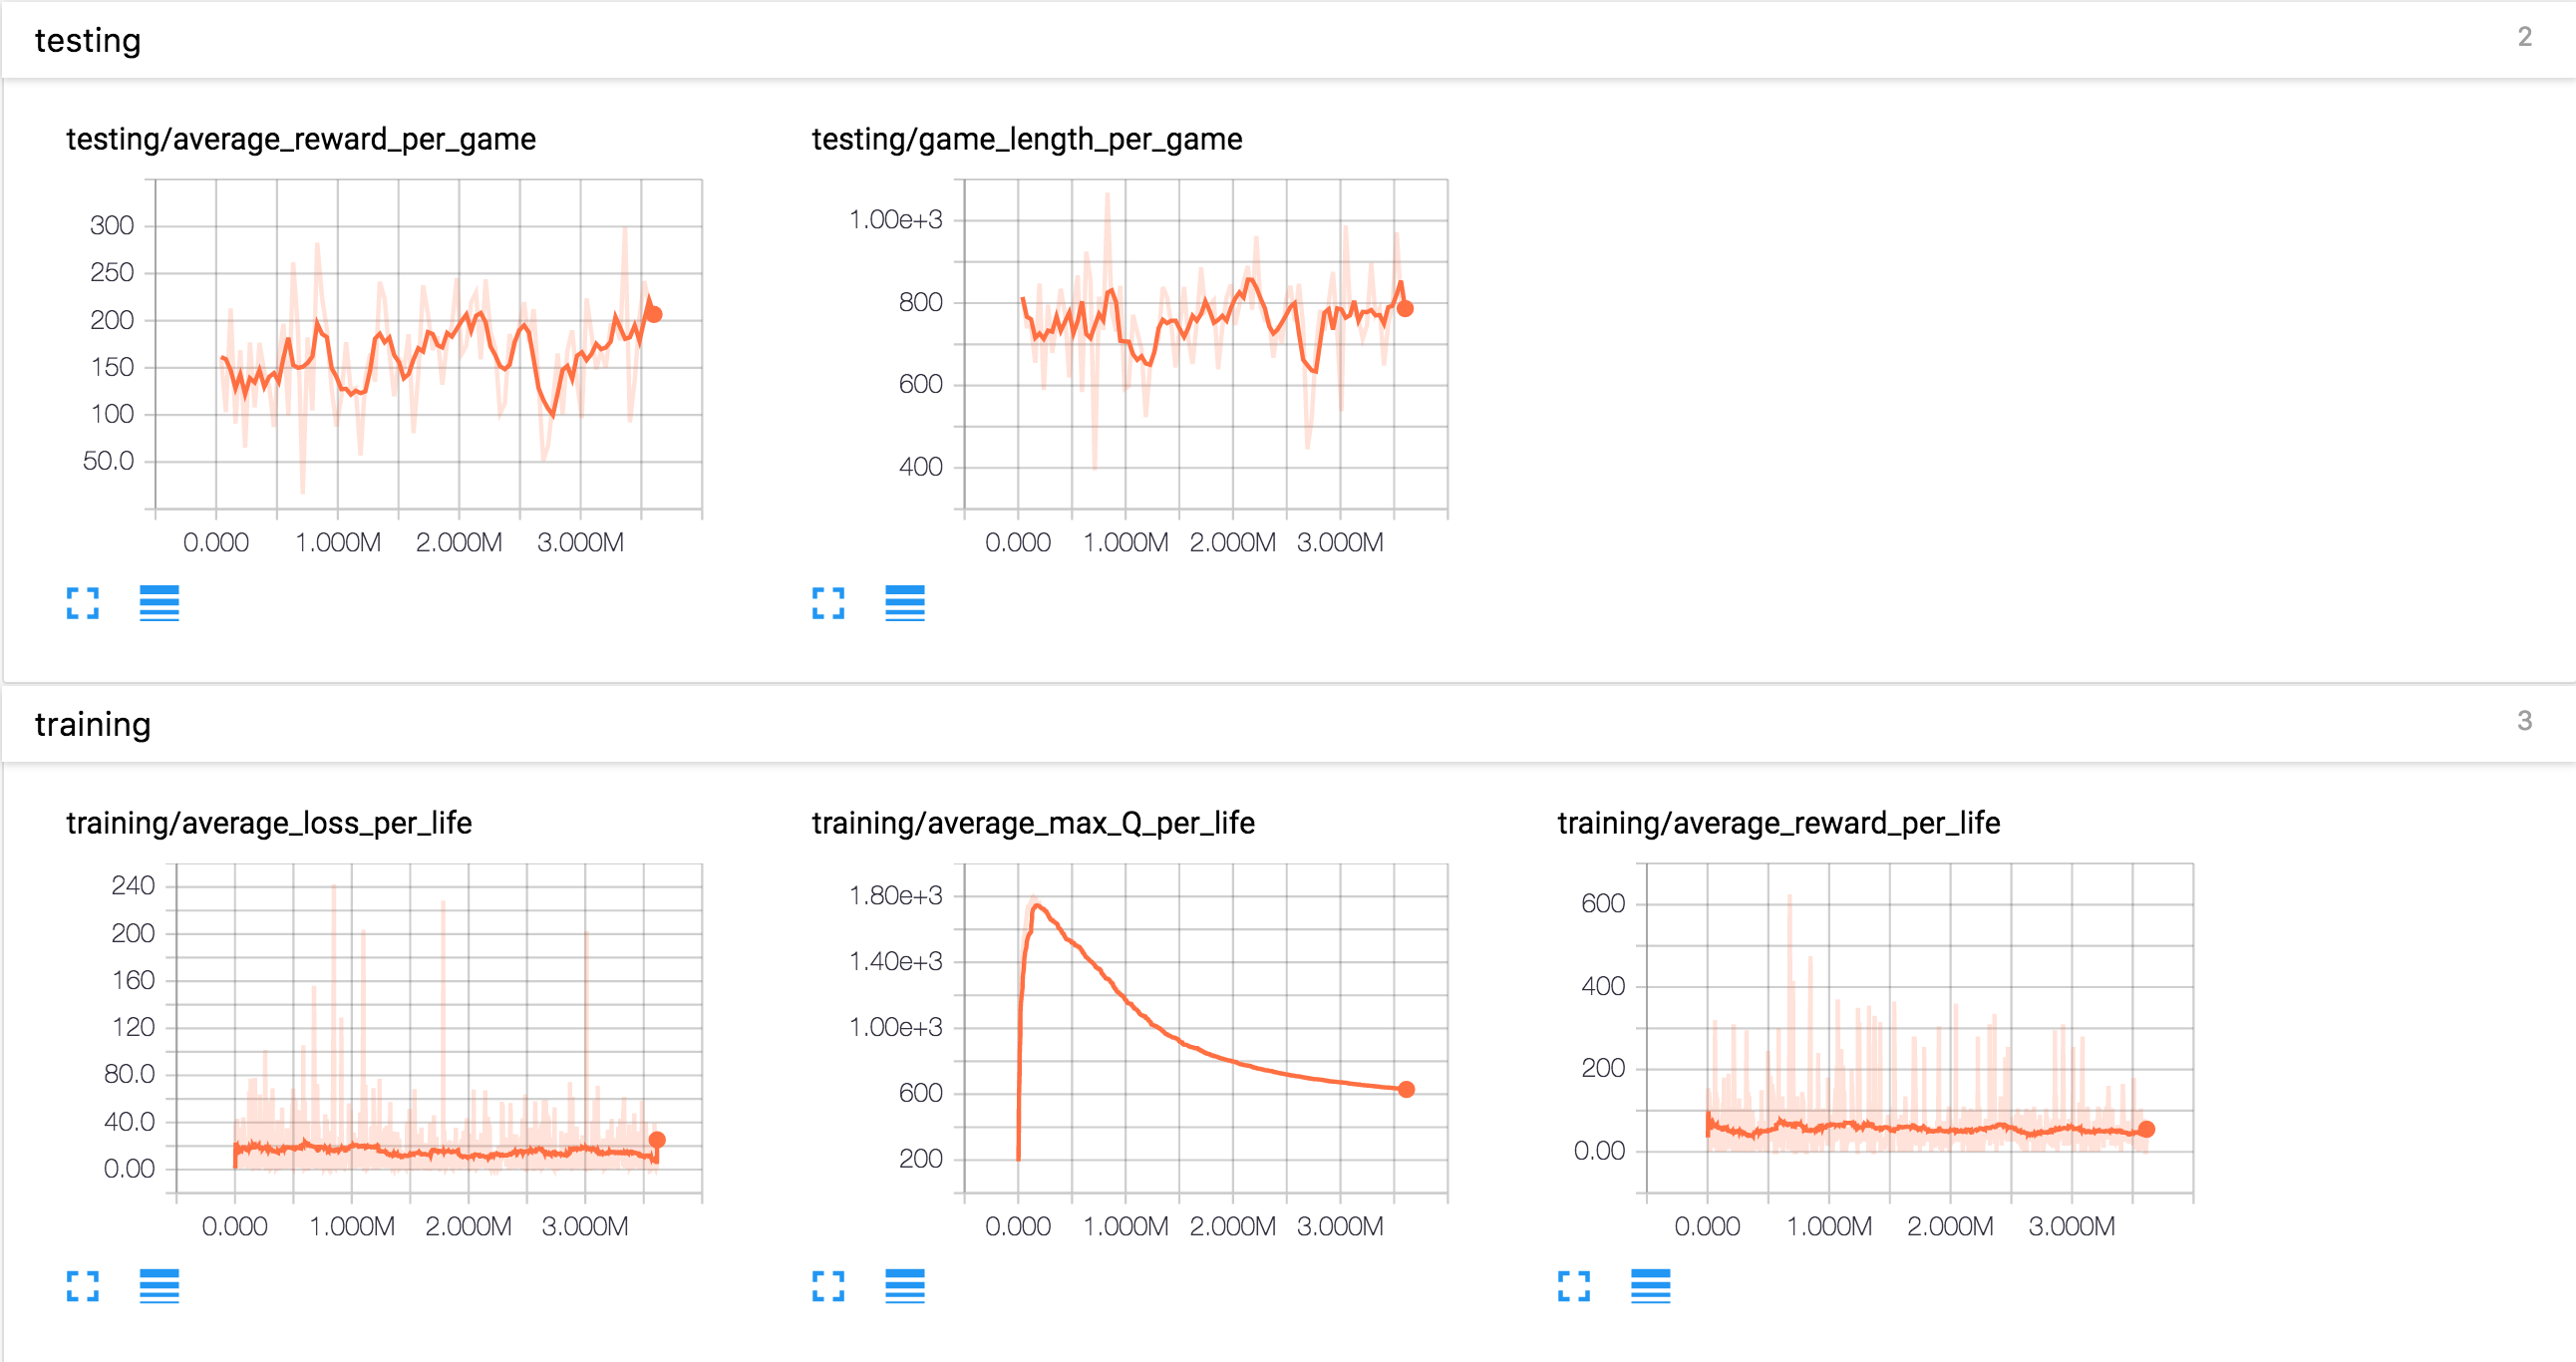
\includegraphics[width=\linewidth]{plots/linear_double.png}
\caption{{\em Double Linear Q-Network:} The progress of max Q value looks similar to what we see in Figure~\ref{fig:linear-simple}. We hypothesize that this is due to {\em no target fixing}. Each network relies on the other one to set the target Q value. However, each network will be updated every 2 iterations in expectation. Hence, this may lead to some unstable training behavior. }
\label{fig:double-linear}
\end{figure}

\begin{figure}[h]
\centering
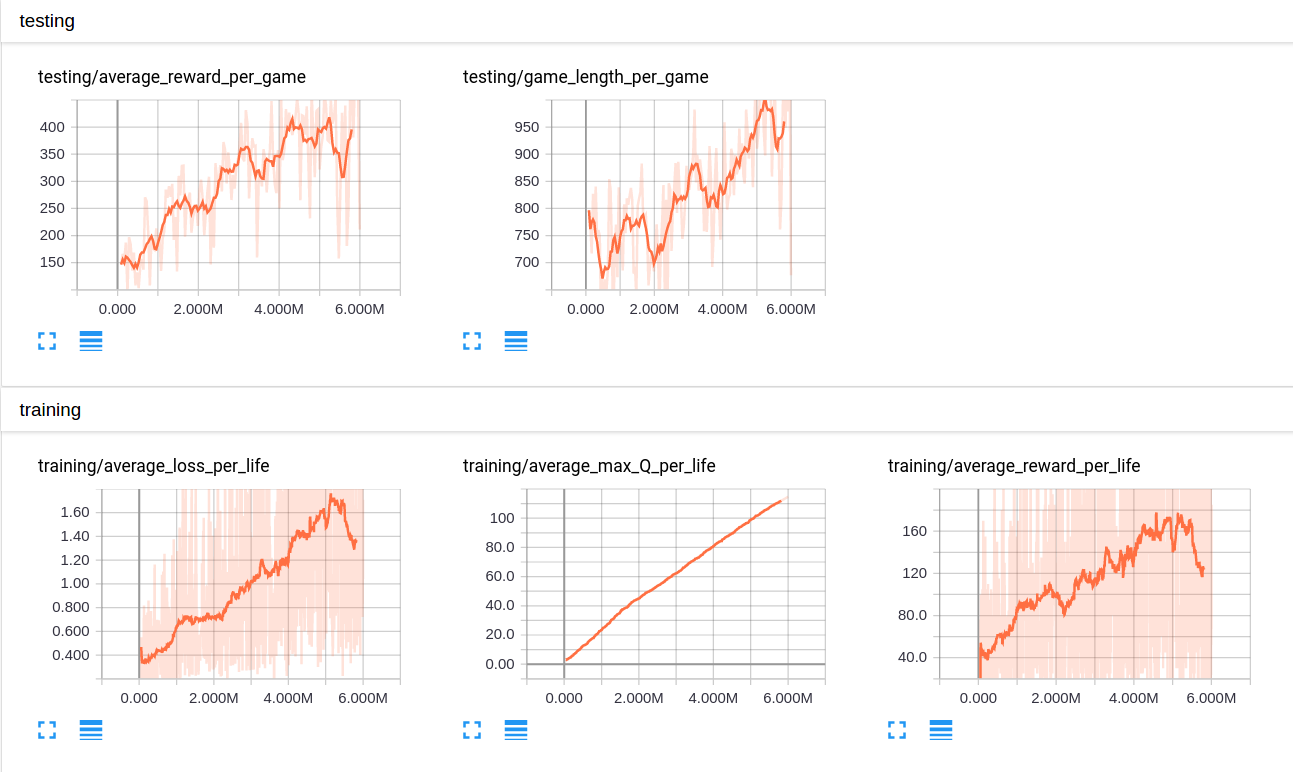
\includegraphics[width=\linewidth]{plots/dqn.png}
\caption{{\em Deep Q-Network:} Both average reward and max Q values go up as expected. }
\label{fig:dqn}
\end{figure}

\begin{figure}[h]
\centering
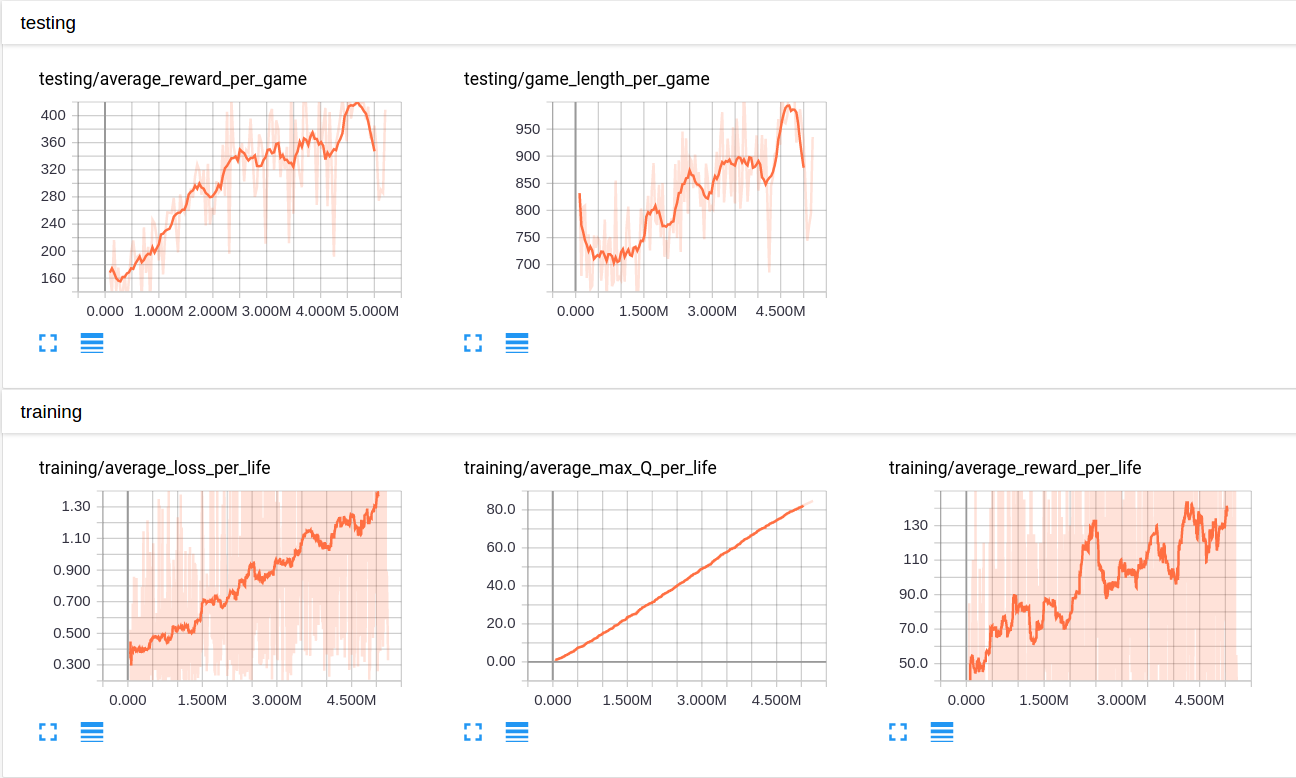
\includegraphics[width=\linewidth]{plots/double.png}
\caption{{\em Double Deep Q-Network:} Both average reward and max Q values go up as expected. }
\label{fig:double}
\end{figure}

\begin{figure}[h]
\centering
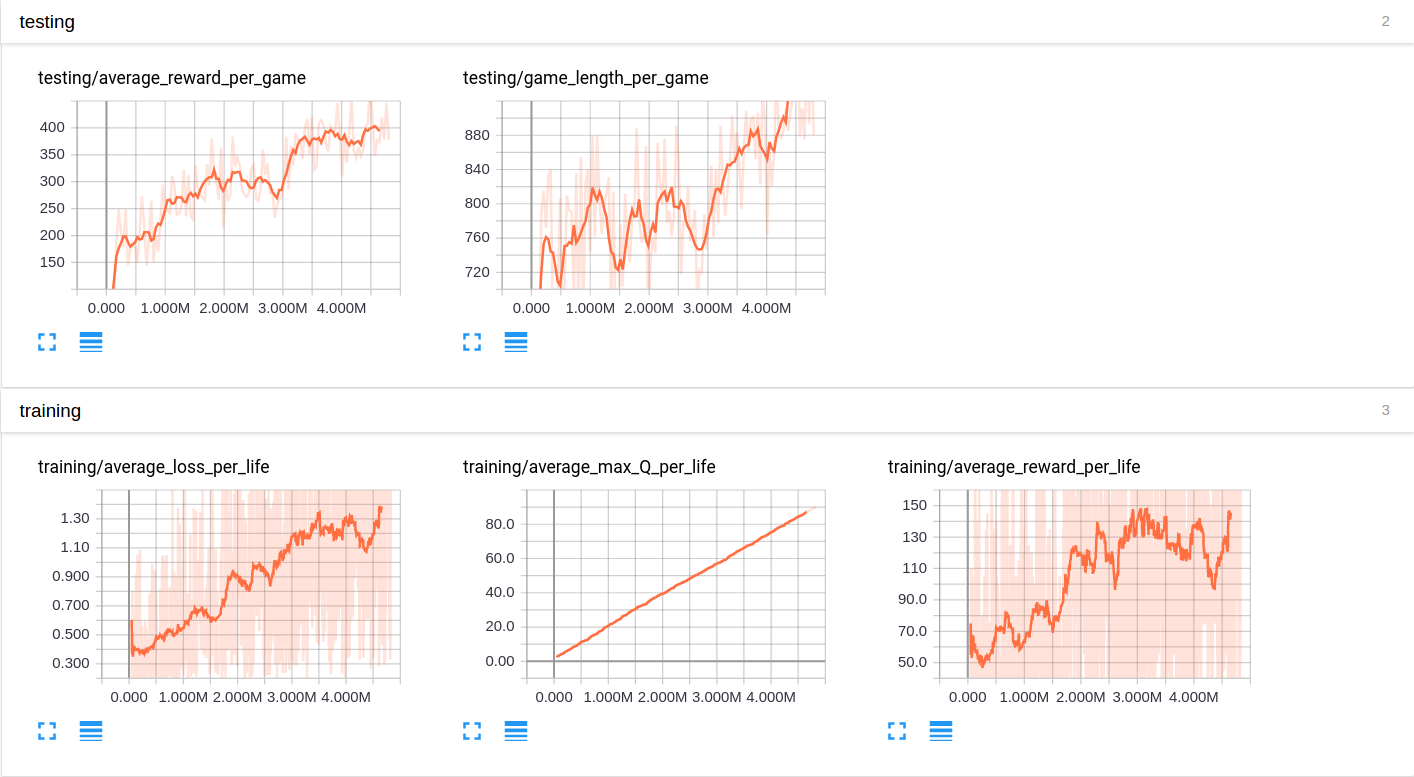
\includegraphics[width=\linewidth]{plots/duel.png}
\caption{{Dueling Deep Q-Network:} Both average reward and max Q values go up as expected. }
\label{fig:duel}
\end{figure}

\subsection{Video captures}
Please find our video captures in a separate submission. 

\subsection{Final performance}
We take the fully trained model of each experiment and run them for 100 episodes. The average accumulative reward per episode for each model is shown in Table~\ref{tab:final}. The results show that:
\begin{itemize}
\item {\em Vanilla DQN} performs better than {\em Double} DQN and {\em Dueling} DQN; 
\item {\em Deep} Q-networks perform generally better than {\em linear} Q-networks;
\item {\em Experience replay and target fixing} are helpful for training a linear Q-network. 
\end{itemize}

\begin{table}
\begin{center}
 \begin{tabular}{||c | c||} 
 \hline
 Model & Average Reward $\pm$ STD. \\ [0.5ex] 
 \hline\hline
 Linear* & 193.15 $\pm$ 83.0 \\
 \hline
 Linear & 225.1 $\pm$ 136.6 \\  
 \hline
 Double-Linear-Q & 159.8 $\pm$ 121.9 \\
 \hline
 DQN & 454.7 $\pm$ 137.3 \\
 \hline
 Double-DQN & 414.3 $\pm$ 140.7 \\  
 \hline
 Dueling-DQN & 362.5 $\pm$ 128.9 \\ 
 \hline
\end{tabular}
\end{center}
\caption{Average rewards and standard deviations for the different network models after for 24 epochs of training (around 5000000 iterations in total). Each epoch includes 50000 network updates. Linear* represents the linear Q-network without experience replay or target fixing. }
\label{tab:final}
\end{table}


\end{document}

%%% Local Variables:
%%% mode: latex
%%% TeX-master: t
%%% End:
